\documentclass[a4paper]{article}
\usepackage{geometry}
\usepackage{graphicx}
\usepackage{apacite,numprint}
\usepackage[utf8]{inputenc}
\usepackage[document]{ragged2e}
\usepackage{xcolor,soul,amsmath}
\title{Report}
\author{Hamid Nazir}
\date{March 2018}
\newcommand{\mathl}[2]{\colorbox{#1}{$\displaystyle #2$}}

\begin{document}

\maketitle

\section{AC susceptibility}

The following incorrect equations were found in \cite{gomory1997characterization}. These equations are valid for $y\leq 1$ only.

\begin{align*}
{\chi}' &=\frac{1}{\pi }\left [  \left ( \frac{y}{2}-1 \right ) \cos^{-1}\left (1- \mathl{gray}{2y}  \right )+ \left( -1 +\frac{4}{3y}-\frac{4}{3y^2} \right ) \left(y-1 \right )^{1/2}\right ]\tag{for slab}\\
{\chi}' &=\frac{\mathl{gray}{2}}{\pi}\left [\left (-1+y-\frac{5y^2}{16}\right ) \cos^{-1}\left ( 1-2y \right )+\left (-\frac{19}{12} + \frac{5y}{8}+\frac{1}{y}-\frac{2}{3y^2}\right ) \left (y-1 \right )^{1/2} \right ] \tag{for cylinder}
\end{align*}

The corrected versions are \cite{goldfarb1991alternating}

\begin{align*}
{\chi}' &=\frac{1}{\pi }\left [  \left (\frac{y}{2}-1  \right ) \cos^{-1}\left (1-\mathl{gray}{\frac{2}{y}}  \right )+ \left( -1 +\frac{4}{3y}-\frac{4}{3y^2} \right ) \left(y-1 \right )^{1/2}\right ]\tag{for slab}\\
{\chi}' &=\frac{\mathl{gray}{1}}{\pi}\left [\left (-1+y-\frac{5y^2}{16}\right ) \cos^{-1}\left ( 1-\mathl{gray}{\frac{2}{y}}\right )+\left (-\frac{19}{12} + \frac{5y}{8}+\frac{1}{y}-\frac{2}{3y^2}\right ) \left (y-1 \right )^{1/2} \right ]\tag{for cylinder}
\end{align*}
\bibliographystyle{apacite}
\bibliography{references}

\newpage
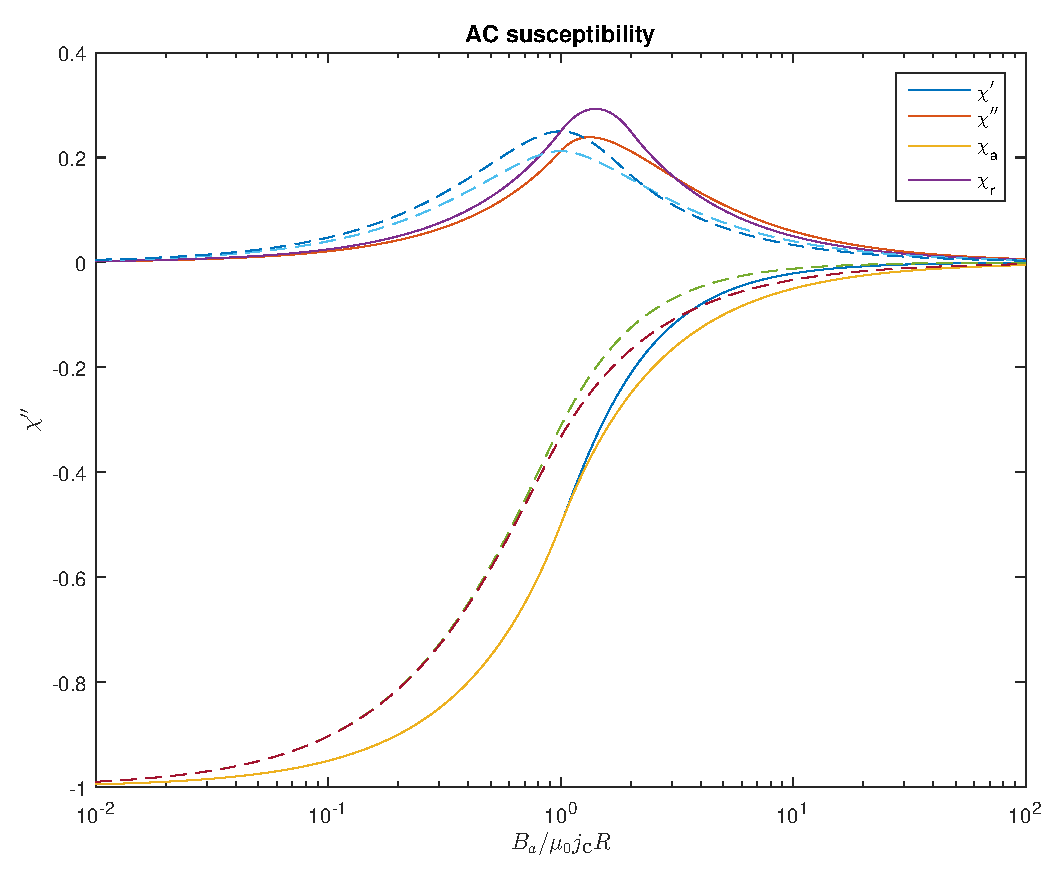
\includegraphics[width=\textwidth]{test_print.eps}
The peak positions are showned in the figure. The following table shows the different maximums at different $y$.
\begin{center}
\npdecimalsign{.}
\nprounddigits{4}
\begin{tabular}{l c n{2}{5} n{2}{5}}
\cline{2-4}
&  & Maximum value & $y$\\
\cline{2-4}
slab&${\chi}''$ &0.238726584205105& 1.33995526965934\\ 
 & $\chi_{\textnormal{r}}$ &0.292872418089059& 1.425102670303\\ \hline
cyliner & ${\chi}''$ &0.212157019811762& 0.984716095793377\\
 & $\chi_\textnormal{r}$ &0.249941600568051 &0.984716095793377\\
\cline{2-4}
\end{tabular}
\npnoround
\end{center}









\end{document}
